% File example.tex
% Contact: simonnet@ecole.ensicaen.fr
%
% version 1.0 (July 24, 2009)
% version 1.1 (September 3, 2009)
% add using of the optional command: \secondauthoraddr

\documentclass[10pt]{article}

% File icdp2009.sty
% Preamble that you have to include to use the template  

% July 24, 2009
% Contact: simonnet@ecole.ensicaen.fr


\usepackage[a4paper,textwidth=18cm,textheight=24cm,top=2.85cm, bottom=2.85cm, left=1.5cm, right=1.5cm]{geometry}

\usepackage{includes/icdp2009}

% left justified caption
\makeatletter
\long\def\@makecaption#1#2{%
\vskip\abovecaptionskip
\sbox\@tempboxa{#1. #2}%
\ifdim \wd\@tempboxa >\hsize
#1. #2\par
\else
\global \@minipagefalse
\hb@xt@\hsize{\box\@tempboxa\hfil}%
\fi
\vskip\belowcaptionskip}
\makeatother




%other package

% vectorial font
\usepackage{lmodern}

\usepackage{graphicx}
\usepackage{times}

\usepackage{textcomp}
\usepackage[justification=centering]{caption}
\usepackage{subcaption}
\usepackage{enumitem}
\usepackage[caption=false]{subfig}
\usepackage{enumitem}
\begin{document}
\noindent

% This should produce references in the order they appear
\bibliographystyle{ieeetr}

%\title{Automatically landmarks prediction on Beetle's pronotum}
%\title{Deep network for landmarks prediction on Beetle pronotums}
%\title{Two scenarios to predict landmarks on Beetle pronotum by Deep Network}
\title{Towards landmarks prediction with Deep Network}

\authorname{Van Linh Le$^{1,3}$, Marie Beurton-Aimar$^{1}$, Akka Zemmari$^1$, Nicolas Parisey$^2$}
\authoraddr{$^1$LaBRI - CNRS 5800 Bordeaux University, France, van-linh.le/beurton/zemmari@labri.fr}

%optional
\secondauthoraddr{$^2$IGEPP - INRA 1349, France, nparisey@rennes.inra.fr }
\thirdauthoraddr{$^3$ITDLU - Dalat University, Vietnam, linhlv@dlu.edu.vn}


\maketitle

\keywords
Landmarks, convolutional neural networks, fine-tuning, recogntion, procrustes.

\abstract
Morphometry landmarks are used in many biological applications. Mostly, the landmarks are defined manually or semi-automatic by applying the image processing techniques. In recent years, deep learning is known as a good solution for the difficult problems in computer vision. It appears in many fields such as classification, recognition, face detection. In the context applying deep learning to solve the regression problems, in this paper, we present a convolutional neural network to predict the landmarks on 2D images, specify beetle's pronotum images. The experiments on the proposed network have been done in two ways: training from scratch and fine-tuning from a trained model. The quality of predicted landmarks is evaluated by calculating the distance in pixels between the coordinates of the predicted landmarks and manual landmarks which were provided by the biologists. The dataset includes $293$ images has been used to experiment the method.

\section{Introduction}
Morphometry landmark (or point of interest) is an important feature in many biological investigations. It was usually used to analyze the forms of whole biological organs or organisms. The analysis is mainly based on the coordinates of the landmarks. The collecting of enough the number of landmarks can help the biologists make a good estimate about organisms. Depending on the problem, the number of landmarks may be more or less; besides, the location of landmarks can be located on the shape (border) or inside the object, \textit{for examples,} the landmarks on Drosophila wings have stayed on the veins of the wings but the landmarks on human ear can be located at the ear hole or inside. Recently, the landmarks were set manually by the biologists. This work is time-consuming and difficult to reproduce. Therefore, a method that proposes automatically the coordinates of landmarks could be a concern. 

Based on the characteristics of digital images acquired for morphological studies, the images can be divided into two groups: the images where they are easy to segment the objects of interest, called \textit{segment-able images}; and the images that we can go in tight when segment the objects, called \textit{un-segment-able images}. For that reason, the methods that used to identify the landmarks automatically may be divided into two groups too. For segment-able images, identification of landmarks on the shape can be finished by applying the image processing techniques such as HOG\cite{palaniswamy2010automatic}, SIFT\cite{lowe2004distinctive}, .... But for un-segment-able images, defining the landmarks become a challenge and the image processing techniques seem to be inappropriate. This article introduces two scenarios for automatic detection of the landmarks on biological images, specific beetle's images. The dataset includes $293$ images of beetles. For each beetle, five parts have been extracted (\textit{pronotum, head, body, left and right mandible}) with their manual landmarks by the biologists. So, the coordinates of the manual landmarks can be seen as the ground truth to evaluated the predicted landmarks.
In this article, a Convolutional Neural Network (CNN)\cite{lecun2010convolutional} has been designed and used in two ways to predict the landmarks: in the first way, the network has been trained from scratch on the dataset of pronotum images. In the second way, the network has been trained on a  ``combination dataset" includes the images of three parts of beetle, firstly; then the trained model was used to fine-tune \cite{yosinski2014transferable} on pronotum dataset. The output model uses to predict the landmarks on a test set of pronotum (Fig.\ref{figpronotum}). 




%The method includes 2 stages: 1) The initially predicted landmarks are given by a convolutional neural network (CNN) \cite{lecun2010convolutional}. The main idea of this stage is design and train a CNN with a set of images and their manual landmarks. The dataset includes $293$ pronotum images and their manual landmarks which have been provided by the biologists. The images are presented in two dimensions and RGB color. After training, the trained network will be able to detect the initially predicted landmarks on the pronotum images; 2) The predicted landmarks which located in the shape of pronotum will be refined the location to increase the accuracy of coordinates. This stage is done by applying a Procrustes analysis\cite{gower1975generalized}. For each manual landmark, a model is generated as a specific. Then, it is used to refine the corresponding predicted landmarks.

\begin{figure}[htbp]
\centering
	\centerline{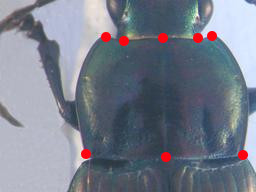
\includegraphics[scale=0.8]{images/pronotum}}
	\caption{An example of pronotum images and its manual landmarks}
	\label{figpronotum}
\end{figure}

In the next section, we present related works in domain automatically estimation landmarks on 2D images. In section 3, we present the architecture of the network and the procedure to generate the data images. Two scenarios to predict the landmarks by using the network are discussed in Section 4. In the last section, we have some conclusion based on the experiments and analyzing the results.

\section{Related works}
Deep learning methods are coming from machine learning theory. They were introduced in a long time ago but the development was still limited. Recently, the improvement of computing capacity, both in memory size and time with GPU programming has opened a new challenge for deep learning. Many deep learning architectures have been proposed to solve the problems of classification \cite{krizhevsky2012imagenet, ciregan2012multi}, image recognition \cite{szegedy2015going, farabet2013learning, li2015convolutional}, speech recognition \cite{mikolov2011strategies, hinton2012deep} and language translation \cite{jean2014using, sutskever2014sequence}. Along with that development, many frameworks have been built such as Caffe \cite{jia2014caffe}, Theano \cite{2016arXiv160502688short}, Tensorflow \cite{tensorflow2015},.... The appearance of the frameworks has helped the users easier to work on deep learning. In image analysis field, deep learning, specifically CNN, is used to predict the key points on the image. Yi Sun et al. \cite{sun2013deep} have proposed a cascaded convolutional network to predict the key points on the human face. Zhang et al. \cite{zhang2014facial} optimizes facial landmarks detection with a set of related tasks such as head pose estimation, age estimation, .... Cintas et al. \cite{cintas2016automatic} have introduced a network to predict the landmarks on human ear images to characterize ear shape. 



In geometric morphometrics, landmarks or points of interest are one of the important characteristics. Landmark studies have traditionally analyzed on 2D images. Depending on which situation was stayed (segment-able or un-segment-able images), setting landmarks must apply the different methods.

When segmentation can be applied, Lowe et al. \cite{lowe2004distinctive} have proposed a method to identify the key points in the 2D image. From the detected key points, the method is able to match two images. Palaniswamy et al. \cite{palaniswamy2010automatic} have applied probabilistic Hough Transform to automatically estimate the landmarks in images of Drosophila wings. Krahenbuhl et al. \cite{le2017maelab} have extended Palaniswamy's method to detect landmarks automatically on beetles mandibles. Unfortunately, this method can not be applied to other parts of beetle that the segmentation has too many noises, such as pronotum images. Fortunately, the applying deep learning sees that a suitable solution to predict the landmarks on un-segment-able images.

%Recently years, machine learning is developing rapidly, specifically deep learning (CNN). It exists in most of the fields, especially in computer vision. We can finish a lot of difficult tasks with a deep convolution neural network such as classification \cite{krizhevsky2012imagenet, ciregan2012multi}, image recognition \cite{szegedy2015going, farabet2013learning, li2015convolutional}, speech recognition \cite{mikolov2011strategies, hinton2012deep} and language translation \cite{jean2014using, sutskever2014sequence}. Using CNN to determine landmarks on 2D images will produce good results and it may be a good solution for the un-segment-able images. Yi Sun et al. \cite{sun2013deep} have proposed a cascaded convolutional network to predict the key points on the human face. Zhang et al. \cite{zhang2014facial} optimizes facial landmarks detection with a set of related tasks such as head pose estimation, age estimation, .... Cintas et al. \cite{cintas2016automatic} have introduced a network to predict the landmarks on human ear images. In the same context, we have applied CNN to predict the landmarks on pronotum images. The predicted landmarks then refined to increase the accuracy of coordinates.

\section{Network model}
Deep learning presents a learning method with multiple levels of representation of connected layers (convolutional neural network). Data representation is transformed from a lower level to a higher level with many complex functions can be learned via backpropagation. In this section, we present a CNN that we have used to predict the landmarks.
\subsection{Network architecture}
\label{secmodel}
The first step to work in CNN is to study the network architecture. After several tests, we have chosen for this application to work with a model provided in Lasagne framework coming from Theano. In the first section, we will present the original model and then, we will describe how we have modified it by definition of an elementary block that we compose in the final model.

Like the networks \cite{lecun2010convolutional, li2015convolutional, cintas2016automatic}, the proposed network consists of common layers with different learnable parameters. It receives an input of $1 \times 256 \times 192$ to train, to validate, and to  test. The network consists of three repeated-structures of a convolutional layer followed by a maximum pooling layer. The depth
of convolutional layers increases with different size of the filter kernels.
All the kernels of pooling layers have the same size. 
At the end, three full connected layers have been added to the
network. %The outputs of the full connected layers are $1000$, $1000$,and $16$, respectively.
 The output of the last full-connected
layer corresponds to 8 landmarks (x and y coordinates) which
we would like to predict. In general way, the layers and their parameters are presented as following:
\begin{itemize}[nosep,label=\footnotesize$\bullet$]
	\item CONV(x,y,z,t): presents for convolutional layer with its parameters: \textit{x = number of filters, y = size of filter matrix, z = stride value, t = padding value},
	\item POOL(y,z,t): presents maximum pooling layer with: \textit{y = size of filter, z = stride value, t = padding value},
	\item FC(x): presents a full-connected layer with \textit{x is the number of output}
\end{itemize}.
Table.\ref{tblmodel1} shows the sequence layers in the model along with the parameters at each layer of the original model.
%\begin{figure}[htbp]
%\centering
%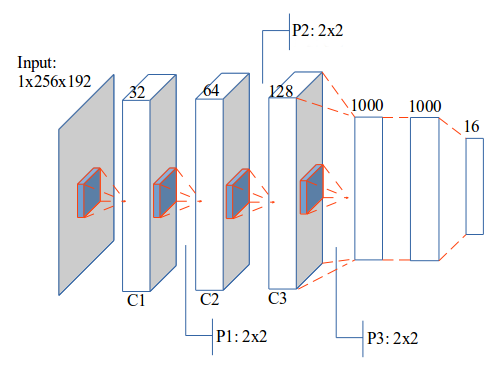
\includegraphics[scale=0.45]{images/architecture1}
%\caption{The first version of the proposed convolutional neural network} 
%\label{cnnnetwork1}
%\end{figure}
\begin{table}[h!]
	
	\begin{subtable}{.22\linewidth}
	\centering
	\begin{tabular}{l l }
	Order & Layer \\ \hline
	1 & Input($1\times256\times192)$ \\ \hline
	2 & CONV(32,3,1,0)\\ \hline
	3 & POOL(2,2,0)\\ \hline
	4 & CONV(64,2,1,0)\\ \hline
	5 & POOL(2,2,0)\\ \hline
	\end{tabular}
	\end{subtable}%
	\hspace{2.8cm}
	\begin{subtable}{.2\linewidth}
	\centering
	\begin{tabular}{l l }
	Order & Layer \\ \hline
	6 & CONV(128,2,1,0)\\ \hline
	7 & POOL(2,2,0)\\ \hline
	8 & FC(1000)\\ \hline
	9 & FC(1000)\\ \hline
	10 & FC(16)\\ \hline
	
	\end{tabular}
	\end{subtable}
	\caption{The layers and their parameters in the original model}
	\label{tblmodel1}
\end{table}

The experiment on original model shows that this architecture is still not good enough to predict the landmarks. It is still general and overfitting has appeared during training and validation.
To prevent the overfitting, four dropout layers have been added into the network. These are considered as the good solution to prevent the overfitting. The idea of dropout is to randomly drop units from the neural network during training \cite{srivastava2014dropout}. Fig.\ref{cnnnetwork2} presents the final architecture of the model. The first three dropout layers are supplemented to the repeated-structures followed the maximum pooling layers. In that way, structure becomes an elementary block includes a convolution layer (\textit{$C_i$}) followed by a maximum pooling (\textit{$P_i$}) and dropout layer (\textit{$D_i$})(with $i=1..3$). The probability values used for dropout layers are $0.1$, $0.2$, and $0.3$. Actually, we keep the same value for the parameters of the convolutional, pooling and full-connected layers as the previous architecture. 
The remaining dropout layer (\textit{$D_4$}) is inserted between the first
two full connected layers (\textit{$FC_1$ and $FC_2$}). The probability value of this layer
is set to $0.5$. The output layer (\textit{$FC_3$}) still contains 16 units corresponding to the coordinates of 8 predicted landmarks.

\begin{figure*}[!t]
\centering
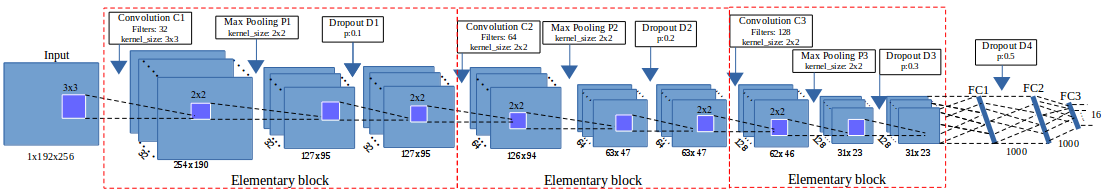
\includegraphics[scale=0.32]{images/arch_model}
\caption{The last version of the proposed convolutional neural network} 
\label{cnnnetwork2}
\end{figure*}

During training, the values of learnable parameters have been updated to increase the accuracy of the network by applying gradient descent in backward phase. Therefore, the network is designed with a small sharing learning rate and momentum. Their values are updated over training time to fit with the number of epochs\footnote{An epoch is a single pass through the full training set.}. The network is designed to finish the training in $5000$ epochs. The learning rate was initialized at $0.03$ and stopped at $0.00001$, while the momentum was updated from $0.9$ to $0.9999$. 
Because landmarks prediction can be seen as a regression problem in deep learning. Therefore, the root mean square error (RMSE) was used as a quality metric to evaluate the result and compute the losses of the proposed architecture. The implementation of the network is done on Lasagne framework \cite{lasagne} which allows computing on GPU. The network has been trained on NVIDIA TITAN X cards.

\subsection{Enlarge the dataset}
\label{sec_data}
The dataset includes $293$ images of beetles (for each part). All images are taken with the same camera in the same condition with a resolution of $3264 \times 2448$. Each image has been set $8$ manual landmarks by biologists (Fig. \ref{figpronotum}). The dataset was split into two subsets: training (and validation) set contains $260$ images and testing set includes $33$ images. In most of CNNs \cite{lecun2010convolutional, sun2013deep,  krizhevsky2012imagenet, cintas2016automatic}, the size of the input is limited to $256$ pixels. In our case, the resolution of input image seems that too large and it becomes a difficulty for the network. So, the images are down-sampling to a new resolution $256 \times 192$ before training and testing. Of course, the coordinates of manual landmarks are also scaled to fit with the new resolution of images.

Besides the size of the input, the number of images is also a challenge when applying CNN. Normally, training a CNN with a large dataset will give us the result better than when we training CNN on a small dataset. Moreover, working with a small dataset, we can meet a popular problem, \textit{overfitting}. So, we need to enlarge the size of the dataset instead of $260$. In image processing, we usually apply transform procedures (translation, rotation) to generate a new image but in fact, when we compute the value of the pixels, it does not change while CNN computes the values of the pixels. To address this problem, we have applied two procedures to enlarge the size of the dataset.

The first procedure is applied to change the value of each
channel in the original image. According to that, a constant is
added to a channel of RGB image and for each time, we just
change the value of one of three channels. For example, from
an original RGB image, if we add a constant c = 10 to the
red channel, we will obtain a new image with the values at
red channel by greater than the red channel of original image
a value of 10. By this way, we can generate three new RGB
images from a RGB image.

The second procedure is splitting the channels of RGB
images. It means that we separate the channels of RGB into
three gray-scale images. This work seems promising because
the network works on single-channel images. At the end of the procedures, we
can generate six versions from an image, the total number of
images used to train and validate is $260 \times 7 = 1820$ images
(six versions and original image).
%\begin{table}[h]
%\begin{center}
%\begin{tabular}{c}
%nn!1 \\
%2 \\
%31 \\
%6 \\
%\end{tabular}
%\end{center}
%\caption{\label{tab1}This is an example of a table caption.}
%\end{table}
%\begin{equation}
%	    PA + A'P - PBR^{-1}B'P + Q  =  0 \enspace.
%\end{equation}


\subsection{First results}
\label{sectrain1}
In this scenario, the network was trained on a dataset of $1820$ pronotum images which were generated from $293$ original pronotum images by applying the procedure in section \ref{sec_data}. The number of images that
used for training and validation is splitted randomly by a ratio
(training: $60\%$, validation: $40\%$) that has been set during the
network setup. During the training, the network learned the information through a pair of \textit{(image, landmarks)} in training set. At the test phase, the image without landmarks was given to the trained network and the predicted landmarks will be given at the output. In practical of CNN, convergence is
usually faster if the average of each input variable over the
training set is close to zero. Moreover, when the input is set
closed with zero, it will be more suitable with the sigmoid
activation function \cite{lecun2012efficient}. According to \cite{lecun2012efficient}, the brightness of
the image is normalized to $[0; 1]$, instead of $[0; 255]$ and the
coordinates of the landmarks are normalized to $[-1; 1]$, instead
of $[0; 256]$ and $[0; 192]$ before giving to the network.



To obtain all the predicted landmarks for all pronotum images (instead of $33$ images), a situation to choose the test images is executed, called \textit{round}. For each round, a set of 33 images have been chosen for the test set; the remaining images have been put into the training set. Following that, the network will be trained with many different training datasets and the output model will be used to predict the landmarks on the images in the corresponding test set. Table.\ref{tbltrainingloss} shows the losses during training the network on pronotum images.

\begin{table}[h!]
	\centering
	\begin{tabular}{l l l}
	Round & Training loss & Validation loss \\ \hline
	1 & 0.00018 & 0.00019  \\ \hline
	2 & 0.00019 & 0.00021 \\ \hline
	3 & 0.00019 & 0.00026 \\ \hline
	4 & 0.00021 & 0.00029 \\ \hline
	5 & 0.00021 & 0.00029 \\ \hline
	6 & 0.00019 & 0.00018 \\ \hline
	7 & 0.00018 & 0.00018 \\ \hline
	8 & 0.00018 & 0.00021 \\ \hline
	9 & 0.00020 & 0.00027 \\ \hline
	\end{tabular}
	\caption{The losses during training the model on pronotum images dataset}
	\label{tbltrainingloss}
\end{table}

Fig.\ref{cnnlosses} shows the training error and the validation error during training time of one round. The blue curve presents RMSE error on training data. The green curve presents the validation error. Clearly, the losses are very different from the beginning. But, the difference is narrowed when the epoch increase.

\begin{figure}[htbp]
\centering
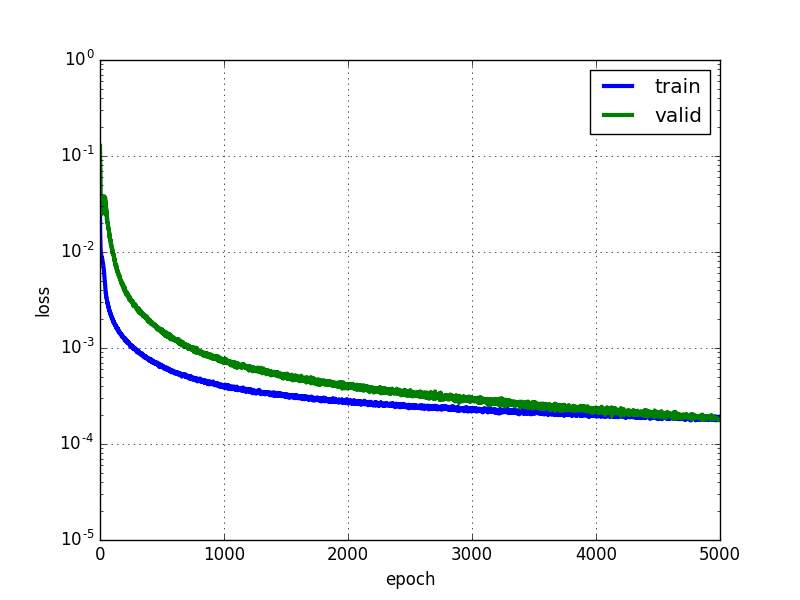
\includegraphics[scale=0.417]{images/losses}
\caption{The loss curves during training of proposed network} 
\label{cnnlosses}
\end{figure}

Besides the losses during training, the accuracy on coordinates of predicted landmarks in the test images is also considered. Firstly, the trained model was used to predict the landmarks on all images in the test set. Then, the distances (in pixels) between manual and corresponding predicted landmarks in each image were calculated as the error distances. Finally, the error distance per landmark was calculated for all test images. Table.\ref{tabledistance} shows the average error distance given on each landmark. With the size of the images is $256 \times 192$, if we accept an error around $3\%$ of the image size ($ \sim3.5$ pixels), the error distances are acceptable.

\begin{table}[htbp]
\centering
\begin{tabular}{|c|p{1.5cm}|}
\hline
\textbf{$\#$Landmark} & \textbf{Distance} \\ \hline
1 & 4.002  \\ \hline
2 & 4.4831 \\ \hline
3 & 4.2959 \\ \hline
4 & 4.3865 \\ \hline
5 & 4.2925 \\ \hline
6 & 5.3631 \\ \hline
7 & 4.636 \\ \hline
8 & 4.9363 \\ \hline
\end{tabular}
\caption{The average error distance per landmark}
\label{tabledistance}
\end{table}
Fig.\ref{figrsexample} shows the predicted landmarks on two test images. When we consider the accuracy of predicted landmarks by calculating the distance between manual and corresponding predicted landmarks, the accuracy on coordinates of predicted landmarks on Fig.\ref{figsub1} is $99\%$ and the propotion on Fig.\ref{figsub2} is $80\%$.

\begin{figure}[htbp]
    \centering
    \begin{subfigure}[t]{0.25\textwidth}
        \centering
        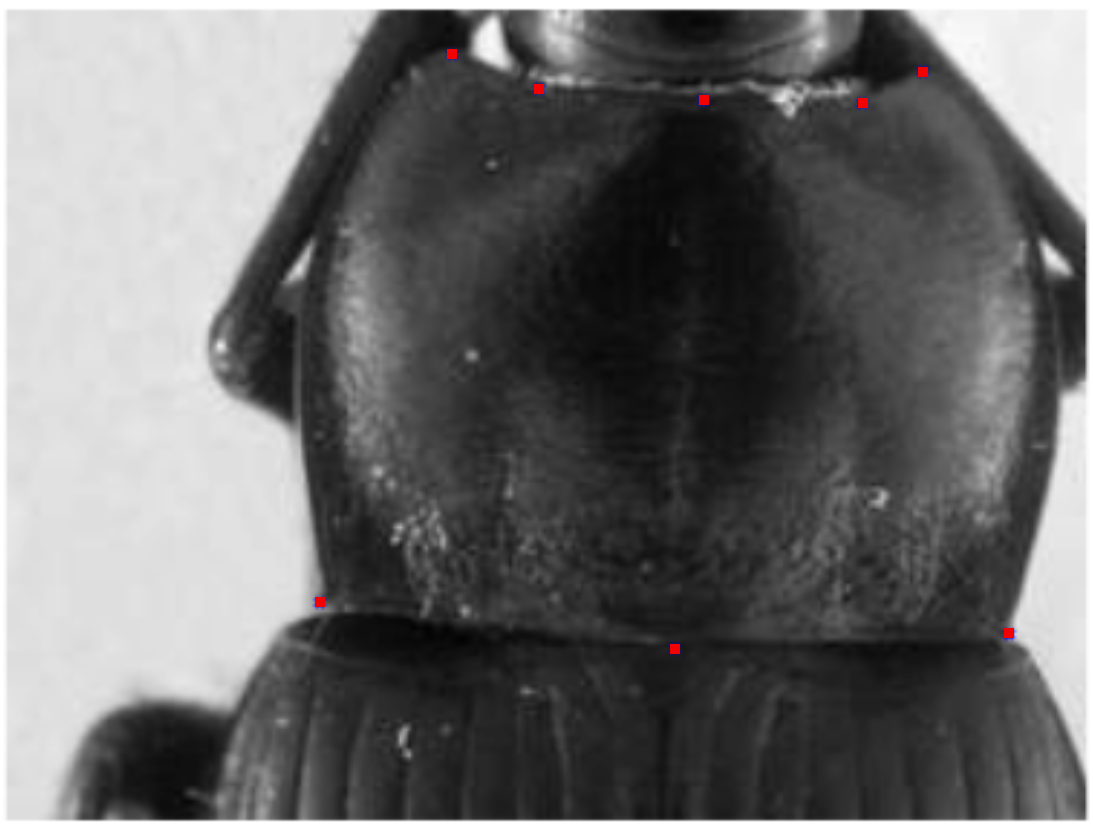
\includegraphics[height=1.2in]{images/plandmark}
        \caption{Image with well-predicted landmarks}
        \label{figsub1}
    \end{subfigure}%
    ~ 
    \begin{subfigure}[t]{0.25\textwidth}
        \centering
        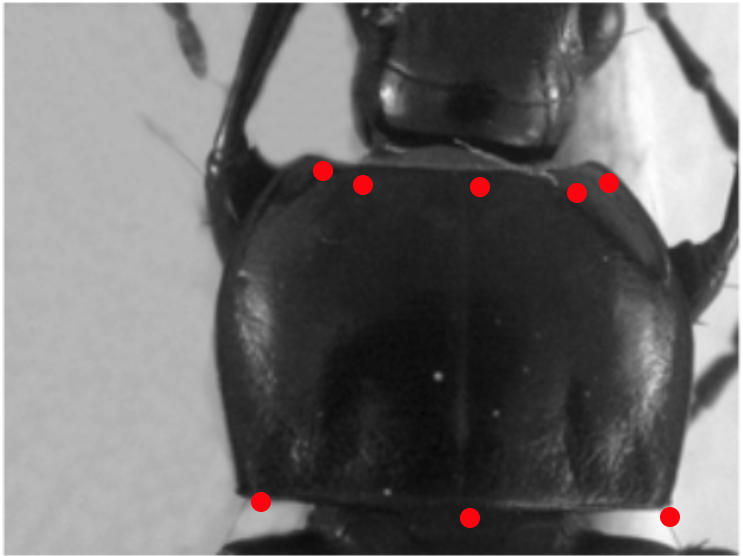
\includegraphics[height=1.2in]{images/plandmark2}
        \caption{Image with inaccuracy landmarks}
        \label{figsub2}
    \end{subfigure}
    \caption{The predicted landmarks on the images in test set.\\
    		 The red points present for the predicted landmarks}
    \label{figrsexample}
\end{figure}

%To have a better evaluation of the predicted landmarks, we have considered the number of acceptable predicted landmarks. In this case, a predicted landmark is considered as acceptable if its error distance to the corresponding manual landmark is less than the average error (per landmark). Fig. \ref{figchart} shows the ratio of acceptable per landmark. Most of landmarks have been predicted with the accuracy grater than \textbf{$80\%$}. In which, the lowest and highest prediction accuracies are \textbf{$83.62\%$} and \textbf{$89.08\%$}, respectively.

%\begin{figure}[htbp]
%	\centerline{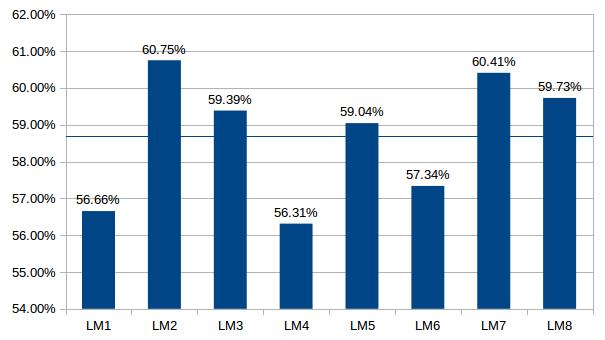
\includegraphics[scale=0.45]{images/avg_chart}}
%	\caption{The proportion of acceptable predicted landmarks}
%	\label{figchart}
%\end{figure}

As a result, the network is able to predict the landmarks on a test set of pronotum images. At statistic side, the predicted landmarks are acceptable. But in image processing side, we expect more about the accuracy (coordinates of predicted landmarks), and the result of CNN is still needed to improve. 
\section{Fine-tuning to transfer learning}
\label{secimproving}
In section \ref{sectrain1}, the proposed network has been experimented by training from scratch on pronotum dataset. The results of experiments have shown that the network has worked well to detect the landmarks on the pronotum images. However, when we consider the predicted landmarks by displaying the landmarks on the images, the result is still not precise, the average error still high ($\geq 4$ pixels). 

In order to reach more acceptable results for biologists, we have broadened the model with the step of transfer learning. That is a method that we re-use the model developed for a task on another task. It allows rapid progress or improved the performance of the model on the second task \cite{torrey2009transfer}. In our case, we have applied fine-tuning, a strategy of transfer learning. Fine-tuning is to not only replace and retrain the model on the new dataset, it also fine-tunes the weight of trained model by continuing the backpropagation. So, instead of training and testing on pronotum images dataset, the network will be trained on the dataset includes the images of three parts of beetle i.e pronotum, body and head. Then, the trained model will be used to fine-tune and test on pronotum set.

%In this section, we describe a scenario to improve the locations of the predicted landmarks which stay at the corner of the pronotum shape, \textit{i.e}  $3^{rd} $ and $7^{th}$ landmarks, called \textit{corner landmarks}. Fig.\ref{figshape} shows the simulation of a pronotum with its shape and manual landmarks. Fig.\ref{figsub11} shows the shape of pronotum and its manual landmarks. The red points represent for the corner landmarks, the yellow points represent the landmarks inside the pronotum. Fig.\ref{figsub22} display an overlap between the shape and real image.

%\begin{figure}[htbp]
%    \centering
%    \begin{subfigure}[t]{0.25\textwidth}
%        \centering
%        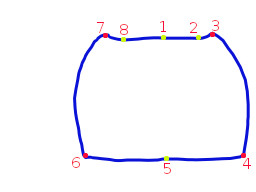
\includegraphics[height=1in]{images/pronotum_model}
%        \caption{Pronotum shape with manual landmarks}
%        \label{figsub11}
%    \end{subfigure}%
%    ~ 
%    \begin{subfigure}[t]{0.25\textwidth}
%        \centering
%        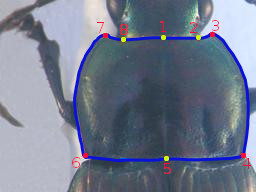
\includegraphics[height=1in]{images/pronotum_overlap}
%        \caption{Overlap the pronotum shape and real image}
%        \label{figsub22}
%    \end{subfigure}
%    \caption{The simulator of a pronotum with its shape } 
%    \label{figshape}
%\end{figure}

%\textit{The main idea of this process is generated a general curve through a landmark and tried to adapt the predicted landmark to corresponding general curve,} this work looks like a Procrustes analysis. The scenario starts from the segmentation result of the image. Firstly, from the training dataset, a ``mean curve" is generated for each manual landmark that stays in the shape of pronotum (i.e $3^{rd}, 7^{th}$). Secondly, for each predicted landmark from CNN, we try to adapt the landmark to the contour of pronotum. Finally, we search a pixel around ``adapted point" that the curve via it is closest to the ``mean curve".

\subsection{Training data preparation}
The training dataset includes a combination of the images from three sets: pronotum, body and head (Fig.\ref{figshape3parts}). For each set, $260$ original images have been chosen radomly for training and validation. By applying the same procedure in section \ref{sec_data}, the training dataset was enlarged to $5460$ images ($260 \times 7 \times 3$). However, the number of manual landmarks on each part is difference: \textit{$8$ landmarks on pronotum part, $11$ landmarks on body part, and $10$ landmarks on head part}. The manual landmarks have a specific meaning for the biologists. So, we can not insert the landmarks arbitrarily. Instead of, we will keep the smallest number of landmarks among three parts and we remove some landmarks on other parts. Therefore, we kept the number of the landmark on pronotum as a reference and we suppressed some landmarks on the body and head part. Specifically, we have removed three landmarks on the body part ($1^{st}; 6^{t}h; 9^{th}$) and two landmarks on the head part ($5{th}; 6^{th}$) (Fig.\ref{figshape3parts}).

\begin{figure}[htbp]
    \centering
    \begin{subfigure}[t]{0.16\textwidth}
        \centering
        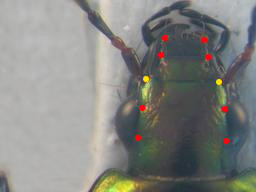
\includegraphics[scale=0.4]{images/ftete}
    \end{subfigure}%
    ~ 
    \begin{subfigure}[t]{0.16\textwidth}
        \centering
        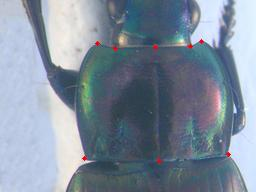
\includegraphics[scale=0.4]{images/fpronotum}
    \end{subfigure}%
    ~
	\begin{subfigure}[t]{0.156\textwidth}
        \centering
        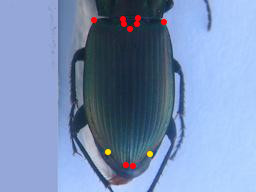
\includegraphics[scale=0.4]{images/felytre}
    \end{subfigure}    
    \caption{The dataset images. The \textit{red} points represent the landmarks that are kept, while \textit{yellow} points represent for the suppressed landmarks during training the model} 
    \label{figshape3parts}
\end{figure}

\subsection{Using fine-tuning for pronotum dataset}
The training data includes $5460$ images was trained on the proposed network (section \ref{secmodel}) with the same parameters than we have trained on pronotum images. After that, the trained model have been continued to fine-tune on pronotum dataset. To compare the result with the previous one, the trained model has been fine-tuned in many rounds with different datasets. The losses during fine-tuning are shown in Table.\ref{tblfinetuningloss}. Comparing with the losses when we trained the model from scratch (Table. \ref{tbltrainingloss}), the validation losses of this scenario are significantly improved (around $40\%$).
\begin{table}[h!]
	\centering
	\begin{tabular}{l l l}
	Round & Training loss & Validation loss \\ \hline
	1 & 0.00019 & 0.00009  \\ \hline
	2 & 0.00018 & 0.00010 \\ \hline
	3 & 0.00018 & 0.00010 \\ \hline
	4 & 0.00019 & 0.00008 \\ \hline
	5 & 0.00019 & 0.00009 \\ \hline
	6 & 0.00018 & 0.00008 \\ \hline
	7 & 0.00019 & 0.00008 \\ \hline
	8 & 0.00018 & 0.00006 \\ \hline
	9 & 0.00018 & 0.00009 \\ \hline
	\end{tabular}
	\caption{The losses during fine-tuning model}
	\label{tblfinetuningloss}
\end{table}

The output model has been used to predict the landmarks on the test images. Then, the average errors based on the distances between predicted and corresponding manual landmarks are given. The results are shown in Table.\ref{tab2}. The \textbf{Error 1} column presents for the average error during training from scratch on pronotum images; the \textbf{Error 2} column presents for the average error during fine-tuning the pronotum from the trained model; and the \textbf{Percentage} column presents for the difference between the distance errors in percentage. Clearly, when we compare the average errors between two scenarios, the result of predicted landmarks in the second scenario is more precise than the first one.

\begin{table}[htbp]
\begin{center}
\begin{tabular}{|c|c|c|c|}
\hline
\textbf{$\#$Landmark} & \textbf{Error 1} & \textbf{Error 2} & \textbf{Improved($\%$)} \\ \hline
\textbf{1} & \textbf{4.002} & \textbf{2.486} & \textbf{37.88} \\ \hline
2 & 4.4831 & 2.720 & 39.33 \\ \hline
3 & 4.2959  & 2.652 & 38.27 \\ \hline
4 & 4.3865  & 2.771 & 36.83 \\ \hline
5 & 4.2925  & 2.487 & 42.06 \\ \hline
\textbf{6} & \textbf{5.3631}  & \textbf{3.049} & \textbf{43.15} \\ \hline
7 & 4.636  & 2.684 & 42.11 \\ \hline
8 & 4.9363  & 2.871 & 41.84 \\ \hline
\end{tabular}
\caption{The average error distance per landmark.}
\label{tab2}
\end{center}
\end{table}

Fig.\ref{figrsexample2} shows the predicted landmarks by applying the second scenario on the same test images as Fig.\ref{figrsexample}. The red points present for the predicted landmarks. In Fig.\ref{figsub11}, the positions of predicted landmarks are the same when we compare with the result from Fig.\ref{figsub1}; but in Fig.\ref{figsub22}, the coordinates of predicted landmarks are strongly improved.
\begin{figure}[htbp]
    \centering
    \begin{subfigure}[t]{0.25\textwidth}
        \centering
        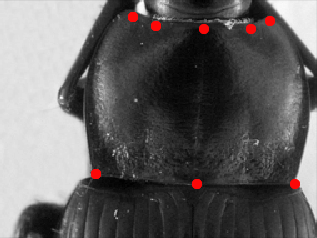
\includegraphics[height=1.2in]{images/fn_accuracy}
        \caption{Image 1}
        \label{figsub11}
    \end{subfigure}%
    ~ 
    \begin{subfigure}[t]{0.25\textwidth}
        \centering
        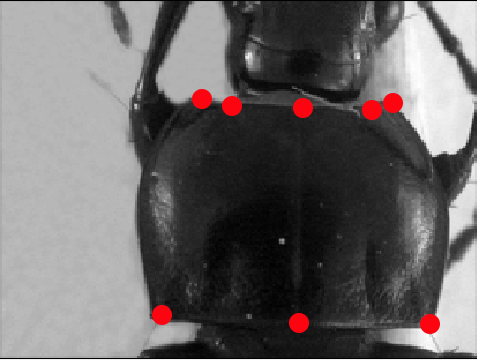
\includegraphics[height=1.2in]{images/fn_inaccuracy}
        \caption{Image 2}
        \label{figsub22}
    \end{subfigure}
    \caption{The predicted landmarks on the images in test set with fine-tuning model.}
    \label{figrsexample2}
\end{figure}

As a result of working, the program outputs the
predicted-landmarks of the images as TPS files. With the outputs are TPS files,
the user can use MAELab framework\footnote{MAELab is a free software written in C++. It can be directly and freely
obtained by request at the authors.} to display the
landmarks on the images.
\section{Conclusion}
In this paper, we have presented a CNN with two scenarios to predict the landmarks on beetle's pronotum images. The CNN network has been designed with three times repeated structure which consists of a convolutional layer, a max pooling layer, and a dropout layer, followed by the connected layers. In the training phase, the CNN have been trained with several times in different selections of training data. After training, the network was able to predict the landmarks on the images in the test set. 

In the first scenario, the model has been trained (from scratch) and tested on the dataset of pronotum images. While in the second scenario, the model has been trained on a dataset includes the images from three parts of beetles. Then, the trained model has been used to fine-tune and test on pronotum images.

The result has been evaluated by comparing the coordinates between predicted and manual landmarks.  The results have shown that using the convolutional network to predict the landmarks on biological images is promising good results in the case that the image was difficult to segment. The quality of prediction allows using automatic landmarking to replace manual landmarks in some aspects. Training model from scratch or fine-tuning the trained model are given the acceptable results. But with a limited number of data, we need to improve the results a little bit. Therefore, future research in landmarking identification appears as an improved of the worth exploring.

\section*{Acknowledgements}
The research has been supported by DevMap project. We would like to thank the my colleague, ALEXIA Marie, who have provided manual landmarks on beetle images.

\bibliography{IEEEabrv,includes/icdp2009}


\end{document}
